\pagebreak
\chapter{Qlik Sense}
\setcounter{section}{0}

\section{Sammelsurium - Qlik Sense}
\subsection{Load} 
\href{https://help.qlik.com/en-US/sense/April2020/Subsystems/Hub/Content/Sense_Hub/LoadData/understand-data-structures.htm}{Load and Select Statment} Was macht den Unterschied aus und wo liegen die Gemeinsamkeiten. 
\begin{lstlisting}[style=Qlik]
	TabellenName:
	Load
	Spaltenname_1,
	Spaltenname_2,
	[
	
	];
\end{lstlisting} 

\subsection{Incremental Loading}
Es ist möglich, nicht eine komplette Datenbank immer und immer wieder zu laden, um an die neuesten Datensätze zu kommen. Es ist möglich, durch \bl{Incremental Loading}. In dem Beispiel, \href{https://youtu.be/wJ0XMmK_5Z4}{Qlik Snippet - Incremental Loading}, wir über einen aufgesetzten SQL-Server gezeigt, wie neue Datensätze geladen werden können.
\begin{itemize}
	\item Erst wir die Initialladung vorgenommen. Diese wird in einem \gls{.qvd} gespeichert.
	\item Im zweiten Schritt wird die Incremental Loading Prozedur vor der Laden-Prozedur geschalten. Diese prüft jetzt, ob in der \gls{SQL} Datenbank neuere Werte als in der dazugehörigen \gls{.qvd} vorliegen. Diese werden dann geladen und in die alte \gls{.qvd} gespeichert.
\end{itemize}


\subsection{Data connection types}
\begin{description}
	\item[Folder] Daten die lokal auf dem Server hinterlegt werden, können so abgerufen werden.
	\item[\gls{ODBC}] Datenbank-Verbindungen, die am Server angelegt werden, können so mit Qlik Sense verbunden werden.
	\begin{figure}[H]
		\centering
		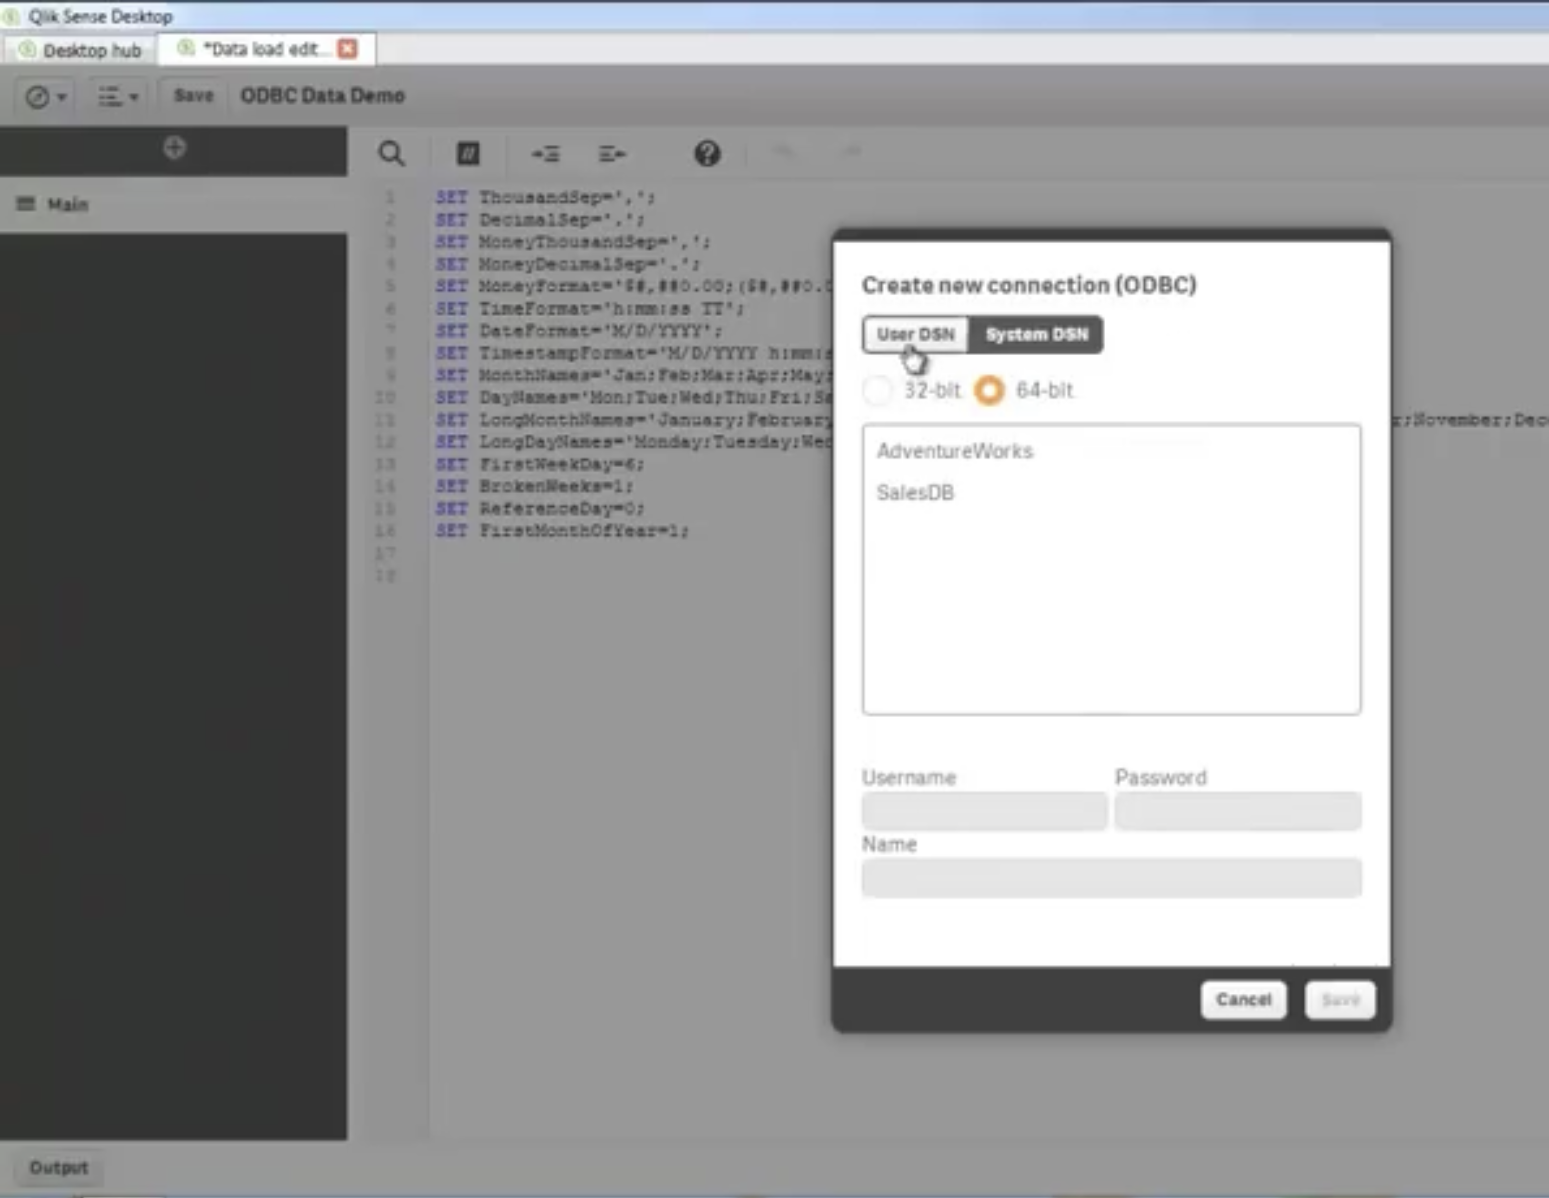
\includegraphics[scale = 0.3]{attachment/chapter_3/Scc008}
		\caption{}
		\label{fig:Scc008}
	\end{figure}
	Qlik bietet an, dass \gls{ODBC} über Qlik Sense direkt angesteuert werden könne oder über Microsoft. 
	\item[Load/ Select] Beide Ausdrücke generieren Tabellen. Dabei wird der Load Ausdruck verwendet, wenn es sich um lokale Dateien handelt. Der Select Ausdruck wird verwendet, wenn Datenbanken adressiert werden. Oft wird dabei auf SQL zurückgegriffen. 
\end{description}

\section{3 - Udemy - Certificate in Qlik Sense Analytics Development}
\subsection{Budgeting and KPI (goal) setting}
\subsubsection{DevHub}
Im Hauptmenü von \gls{g_QlikSense} kann die DevHub Umgebung angesteuert werden.

\begin{figure}[H]
	\centering
	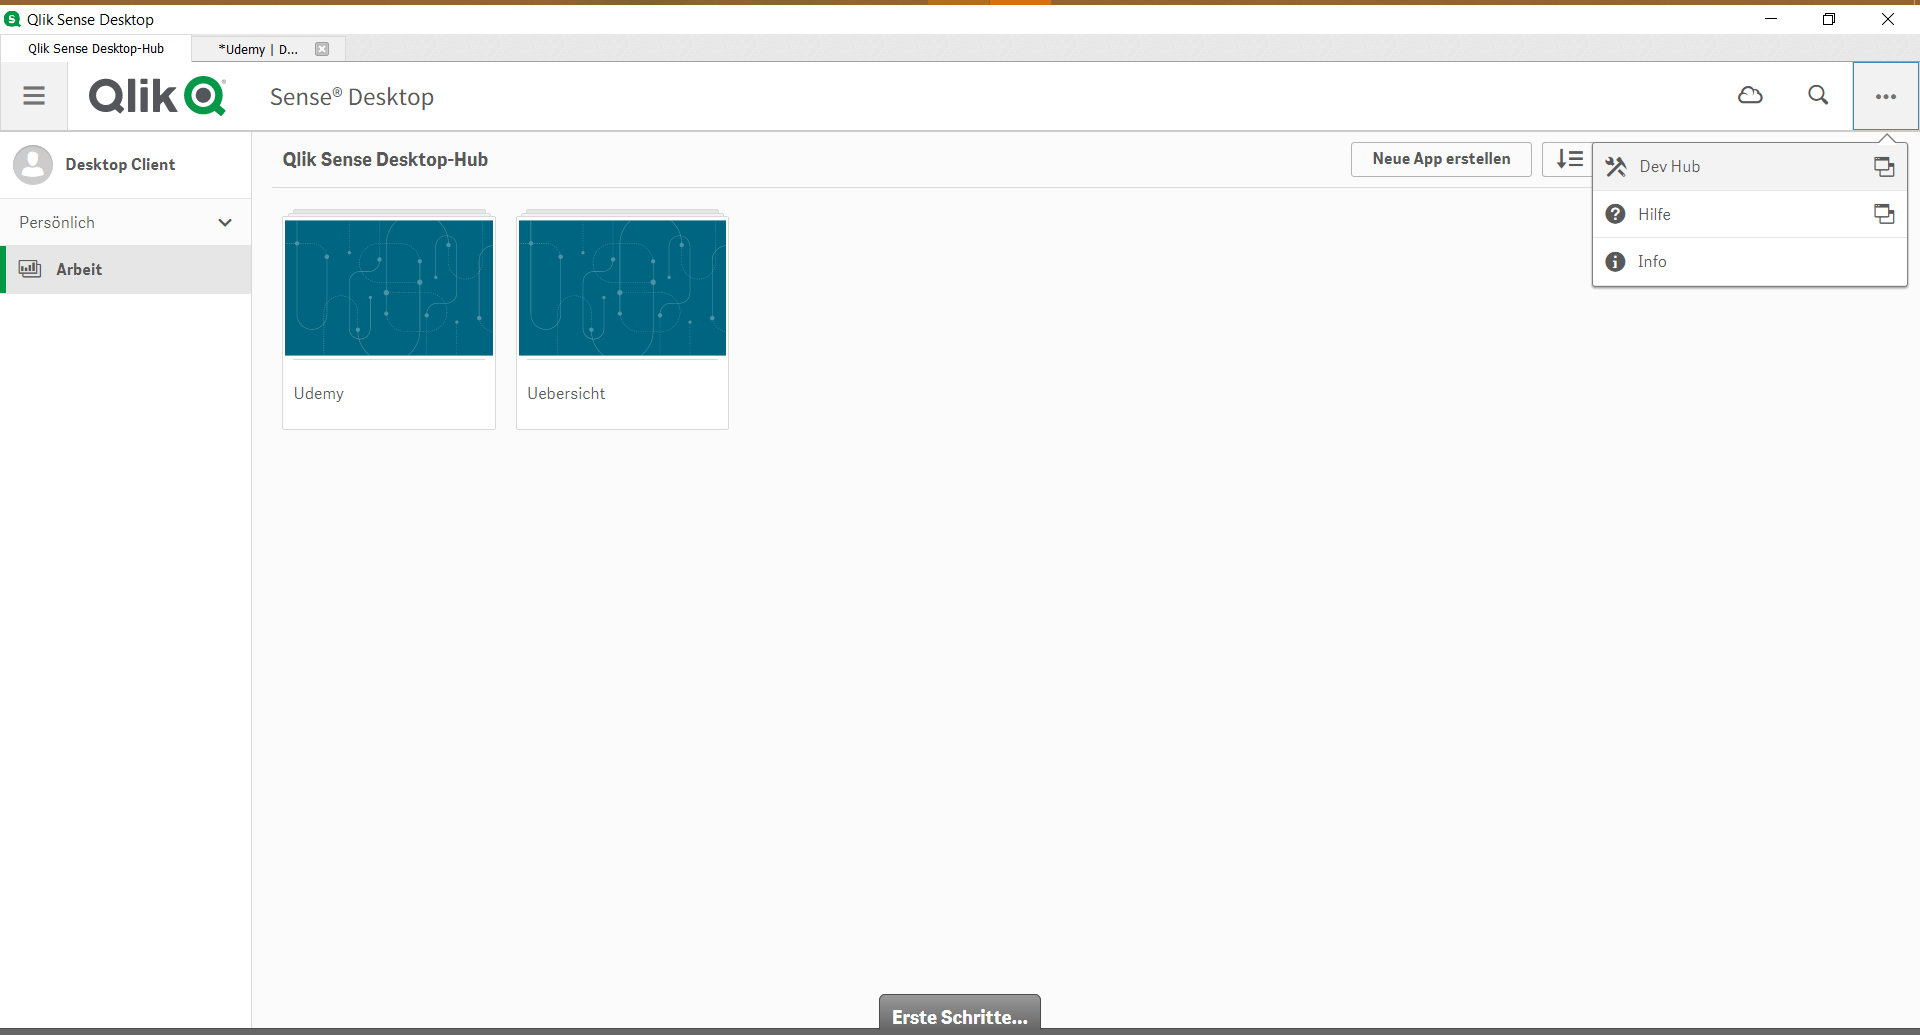
\includegraphics[scale = 0.3]{attachment/chapter_3/Scc009}
	\caption{}
	\label{fig:Scc009}
\end{figure}
Diese bietet an
\begin{itemize}
	\item MashUps, 
	\item Erweiterungen von Visualisierungen und
	\item Widget zur Verfügung zu stellen.
\end{itemize}

\begin{figure}[H]
	\centering
	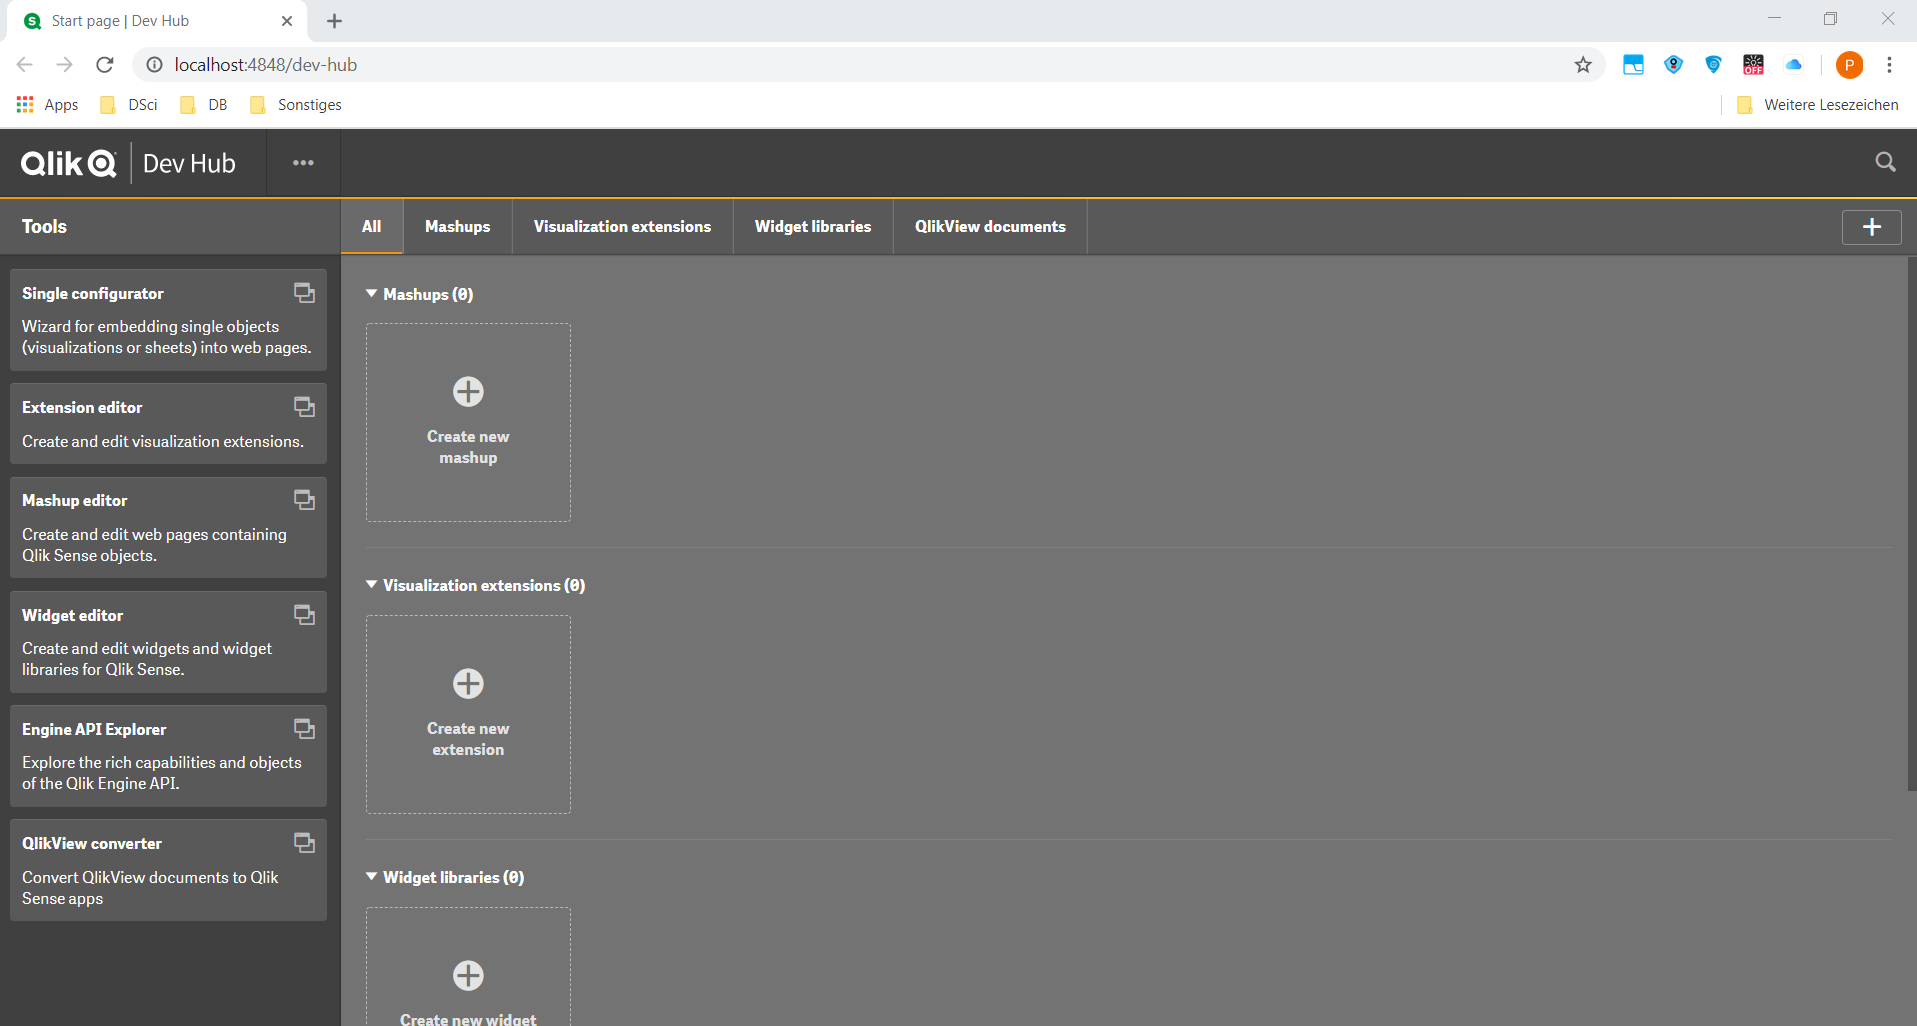
\includegraphics[scale = 0.3]{attachment/chapter_3/Scc010}
	\caption{}
	\label{fig:Scc010}
\end{figure}
Wichtige Punkte sind:
\begin{itemize}
	\item Diese Features werden verwendet, um sie in andere Umgebungen einzubinden. Mashups werden so verwendet, um sie in SharePoint einzubinden.
	\item Die Plattform \href{www.branch.qlik.com}{Qlik Branch} gibt eine Übersicht über die verschiedenen Anbindungsmöglichkeiten zu \gls{g_QlikSense}.
	\item Visualisierungserweiterungen werden über \gls{JS} programmiert.
\end{itemize}
\subsubsection{Von Hub bis Sheet}
Die Hub Oberfläche unterscheidet sich von dem \gls{QMC}, dass die Datenaufbereitung über diese Oberfläche zur Verfüugng gestellt wird und \gls{QMC} die Verwaltung übernimmt.
\begin{description}
	\item[Stream] In einem Stream können mehrere Apps veröffentlicht werden. Die Berechnungen wird über die Stream festgelegt.
	\item[Apps] In einer App wird die Datengrundlage bestimmt. Das zugrundeliegende Datenmodell dient den Sheets.
	\item[Sheets] Über Sheets können Visualierungen erstellt werden.
\end{description}

\begin{figure}[H]
	\centering
	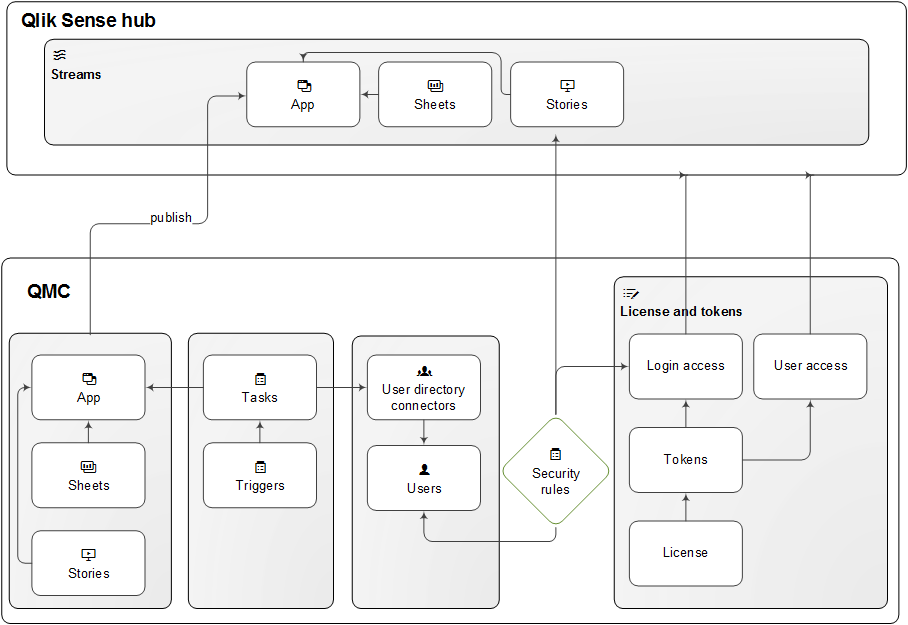
\includegraphics[scale = 0.3]{attachment/chapter_3/Scc015}
	\caption{}
	\label{fig:Scc015}
\end{figure}
Am Beispiel des Streams \textbf{Arbeit} wird die App \textbf{Udemy} erstellt.

\begin{figure}[H]
	\centering
	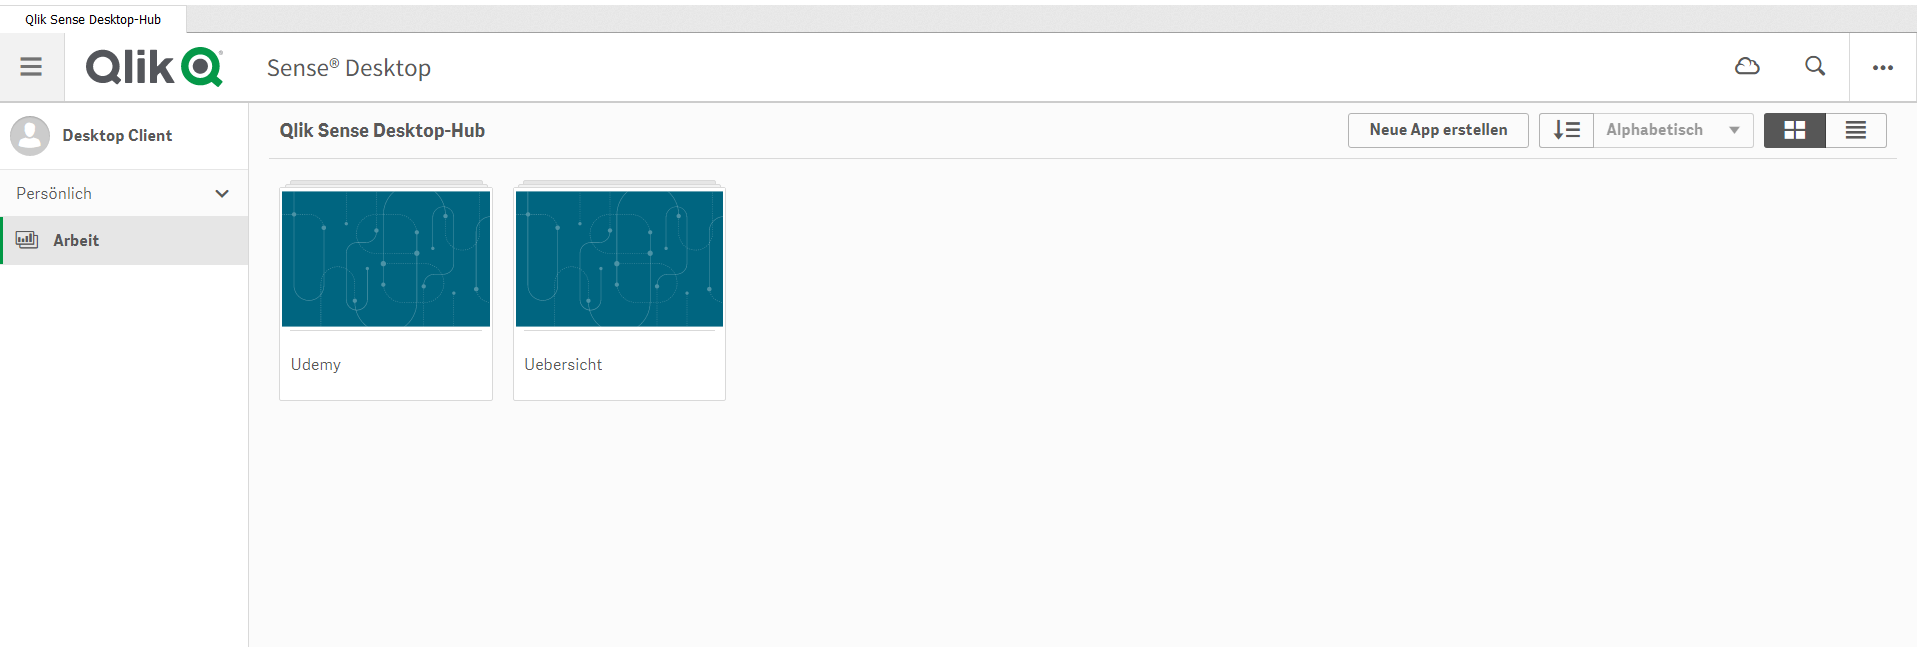
\includegraphics[scale = 0.3]{attachment/chapter_3/Scc011}
	\caption{}
	\label{fig:Scc011}
\end{figure}

Beim Öffnen der App erscheint die der Datenmanager.

\begin{figure}[H]
	\centering
	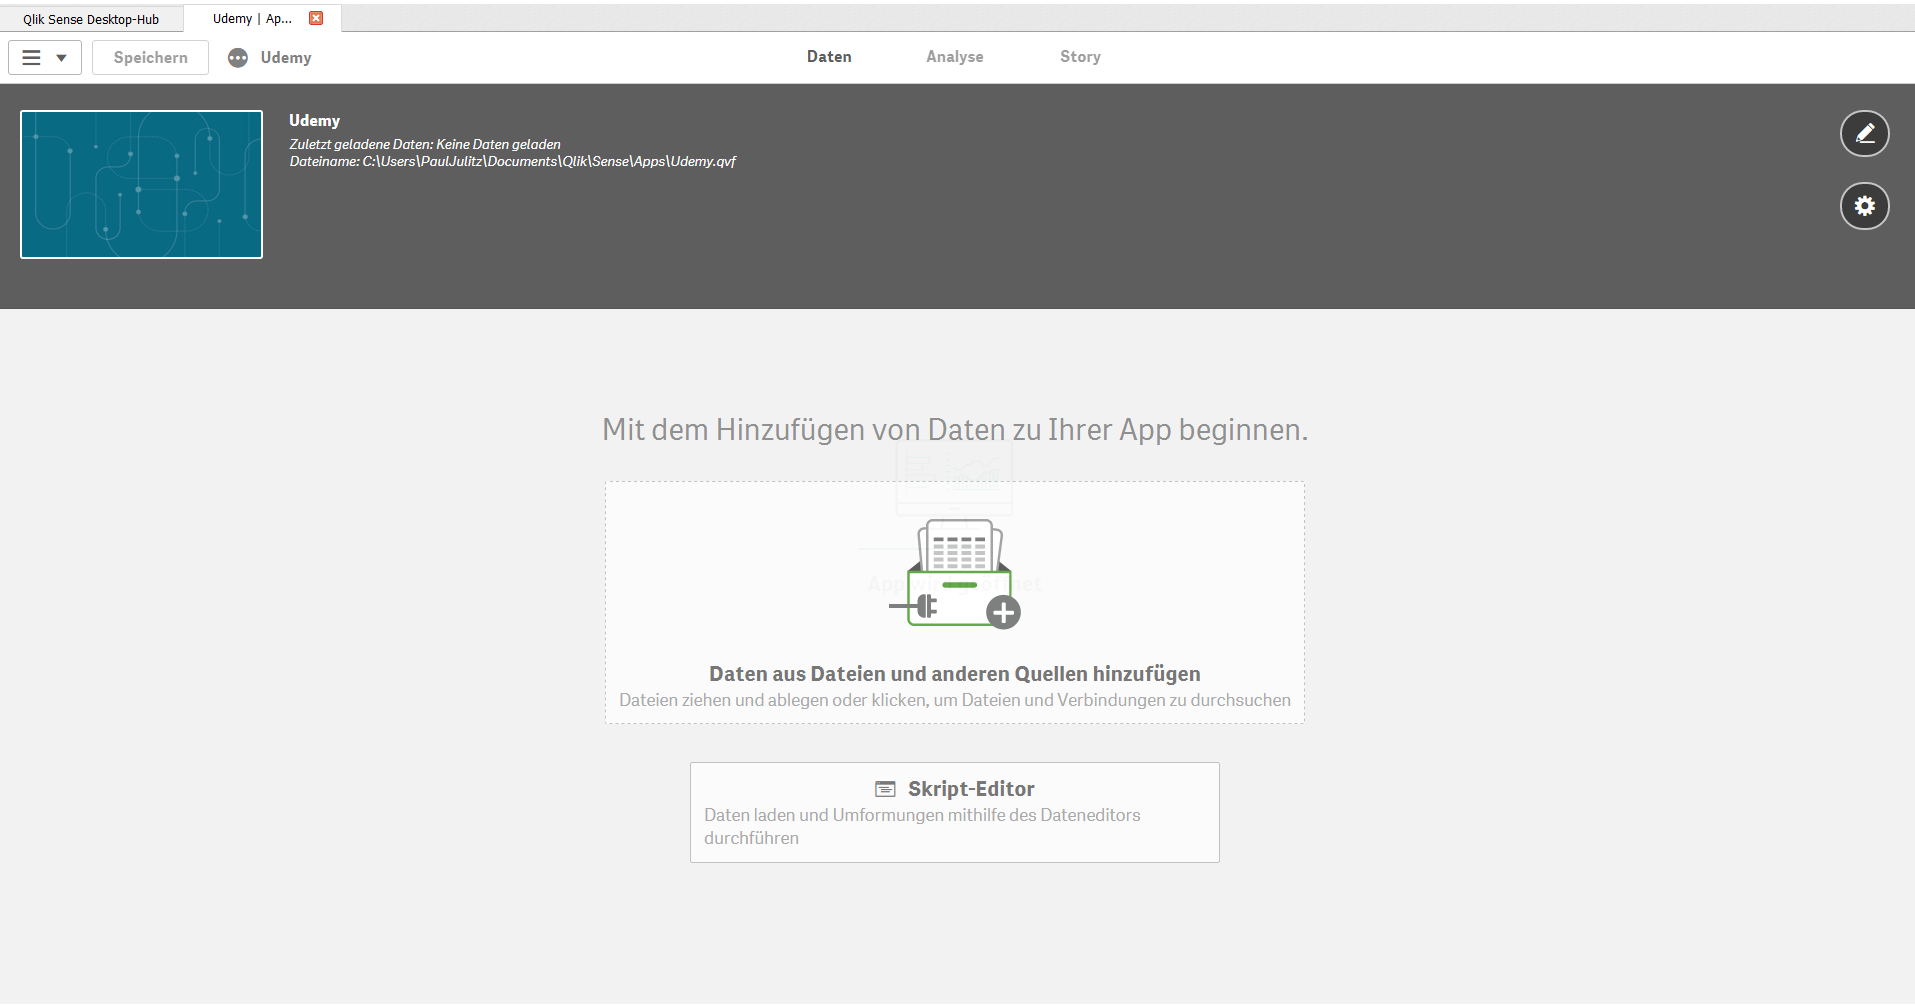
\includegraphics[scale = 0.3]{attachment/chapter_3/Scc012}
	\caption{}
	\label{fig:Scc012}
\end{figure}
Über diesen können verschiedenen Verbindung angesteuert werden.

\begin{figure}[H]
	\centering
	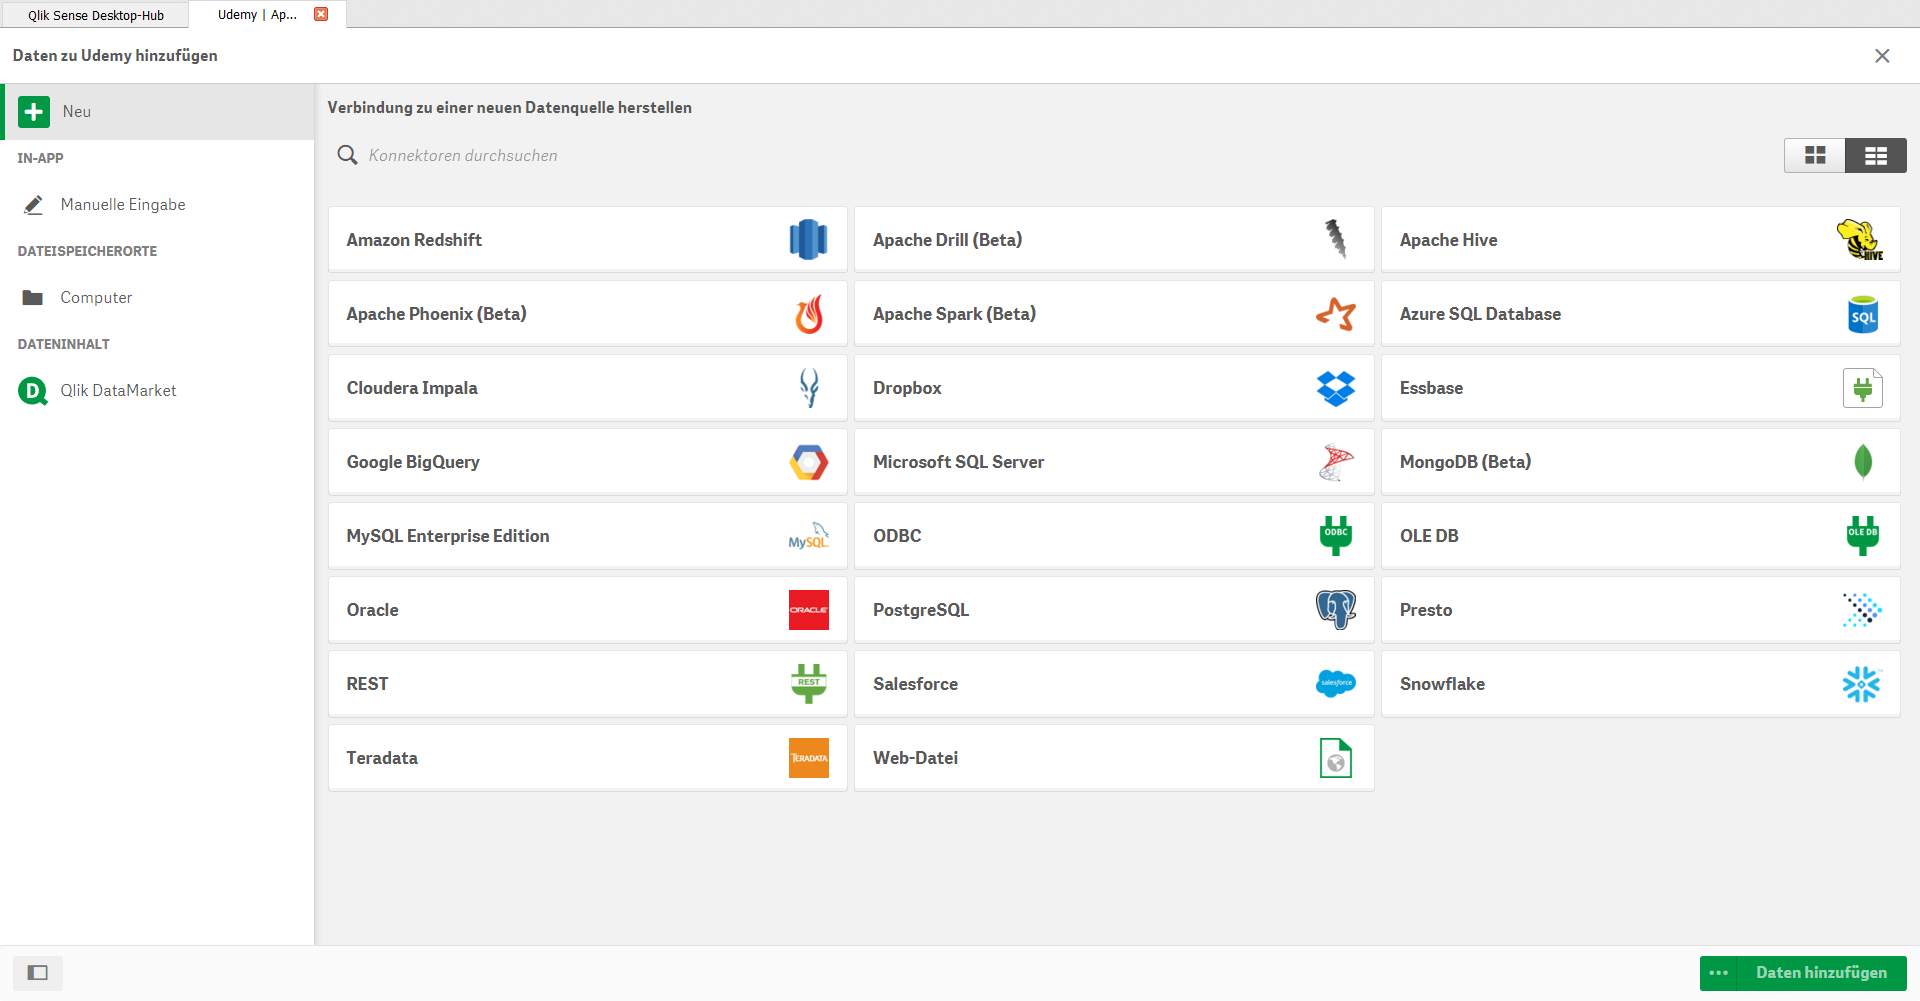
\includegraphics[scale = 0.3]{attachment/chapter_3/Scc013}
	\caption{}
	\label{fig:Scc013}
\end{figure}
Wird auf lokale Dateien zugegriffen, sieht das wie folgt aus:

\begin{figure}[H]
	\centering
	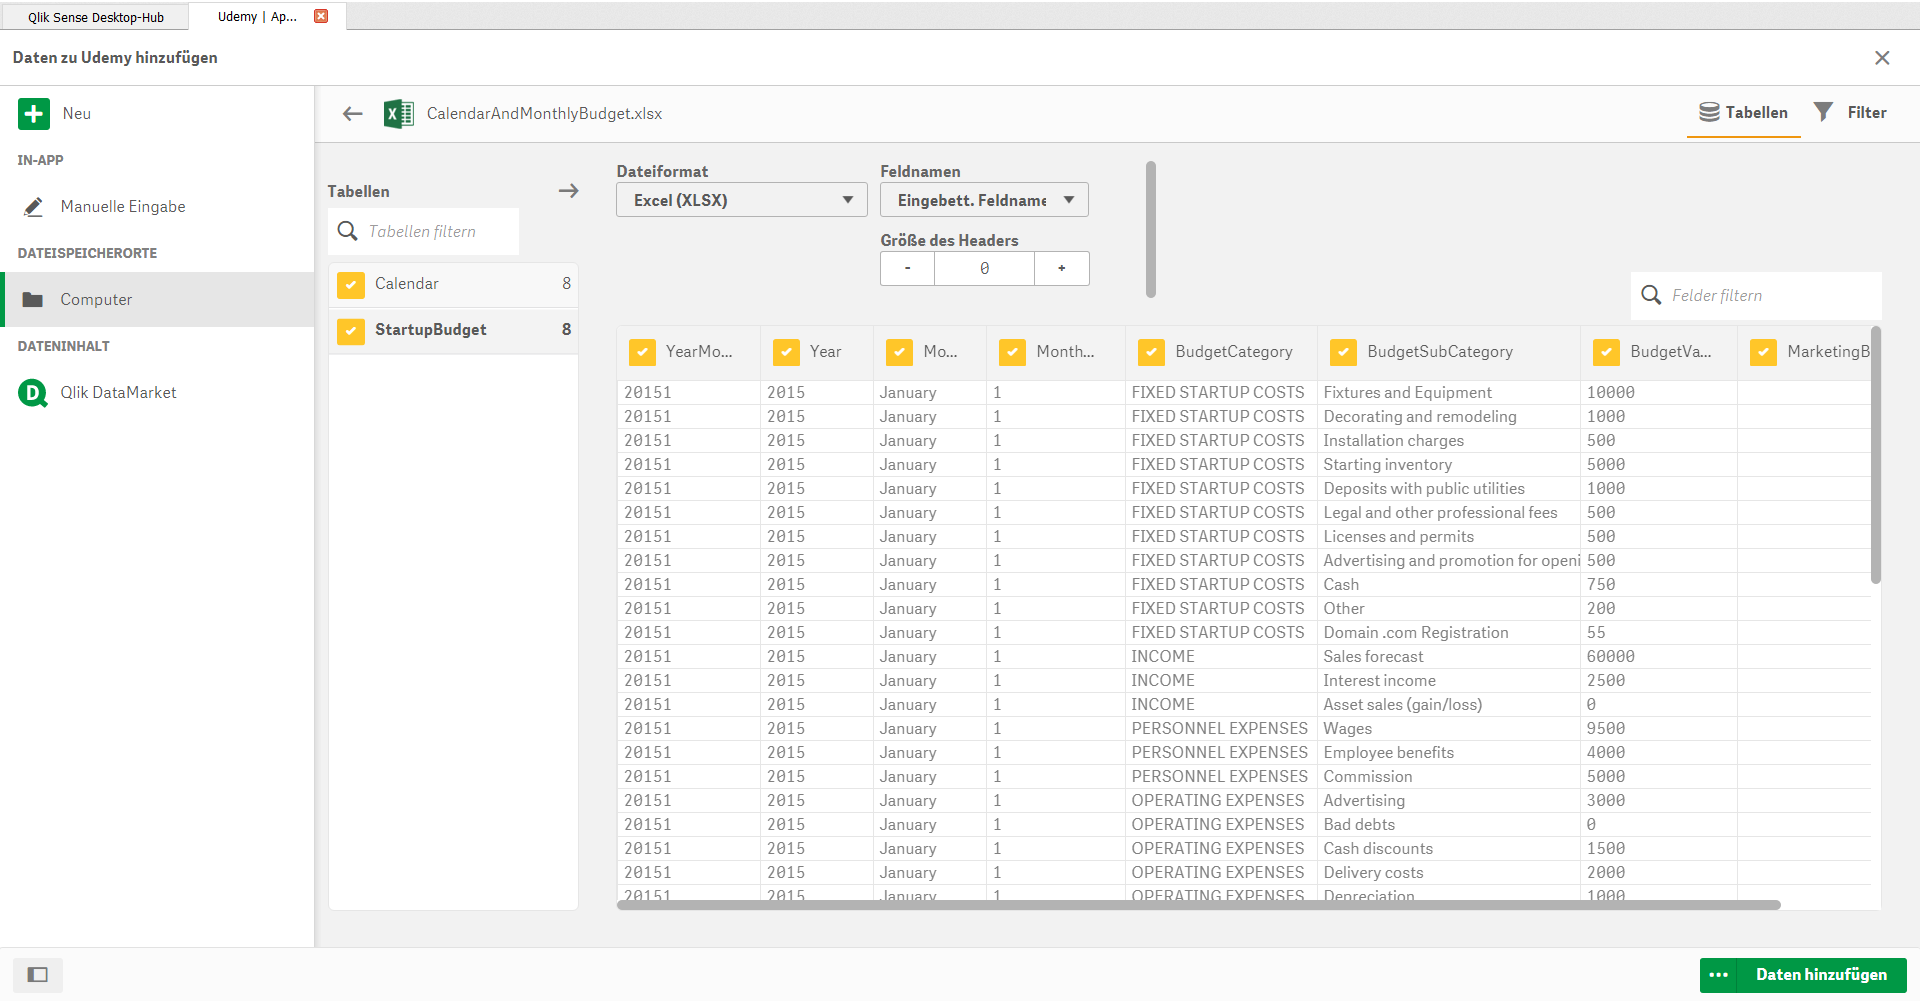
\includegraphics[scale = 0.3]{attachment/chapter_3/Scc014}
	\caption{}
	\label{fig:Scc014}
\end{figure}

Nachdem die Daten geladen werden.
\begin{figure}[H]
	\centering
	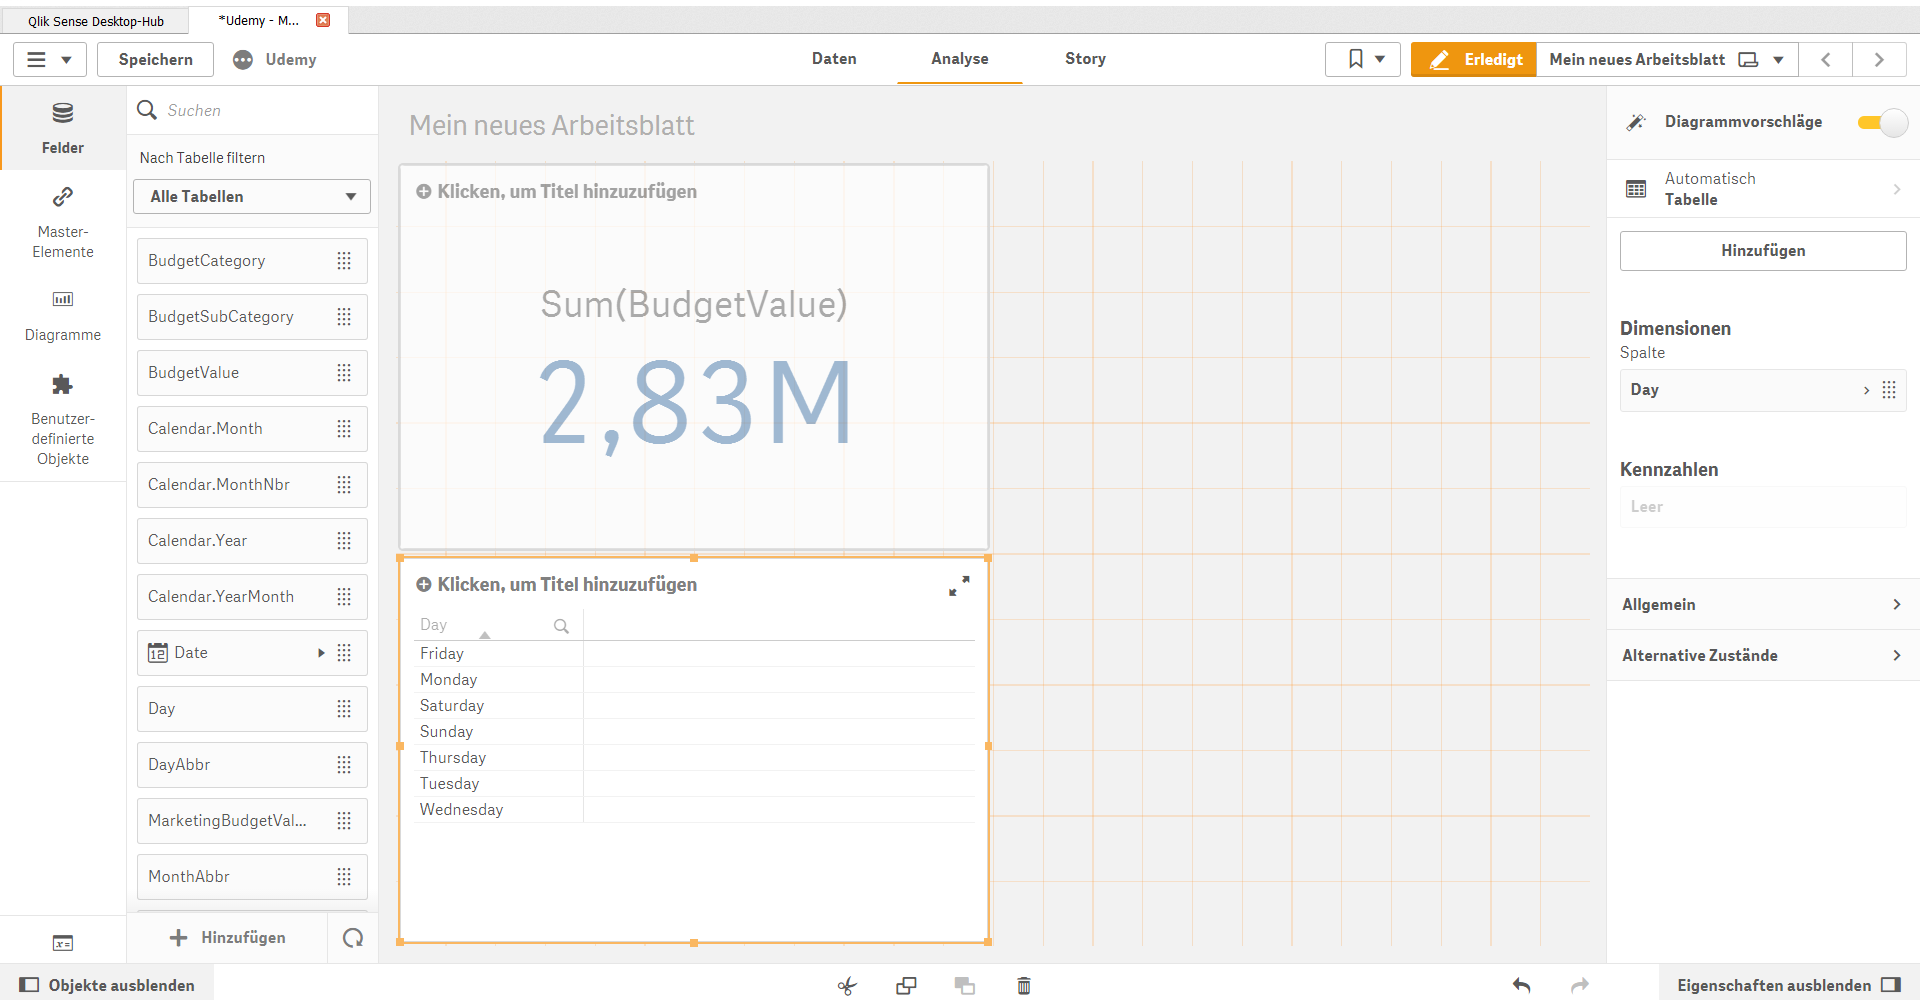
\includegraphics[scale = 0.3]{attachment/chapter_3/Scc016}
	\caption{}
	\label{fig:Scc016}
\end{figure}

kann ein neues Arbeitsblatt angelegt werden.
\begin{figure}[H]
	\centering
	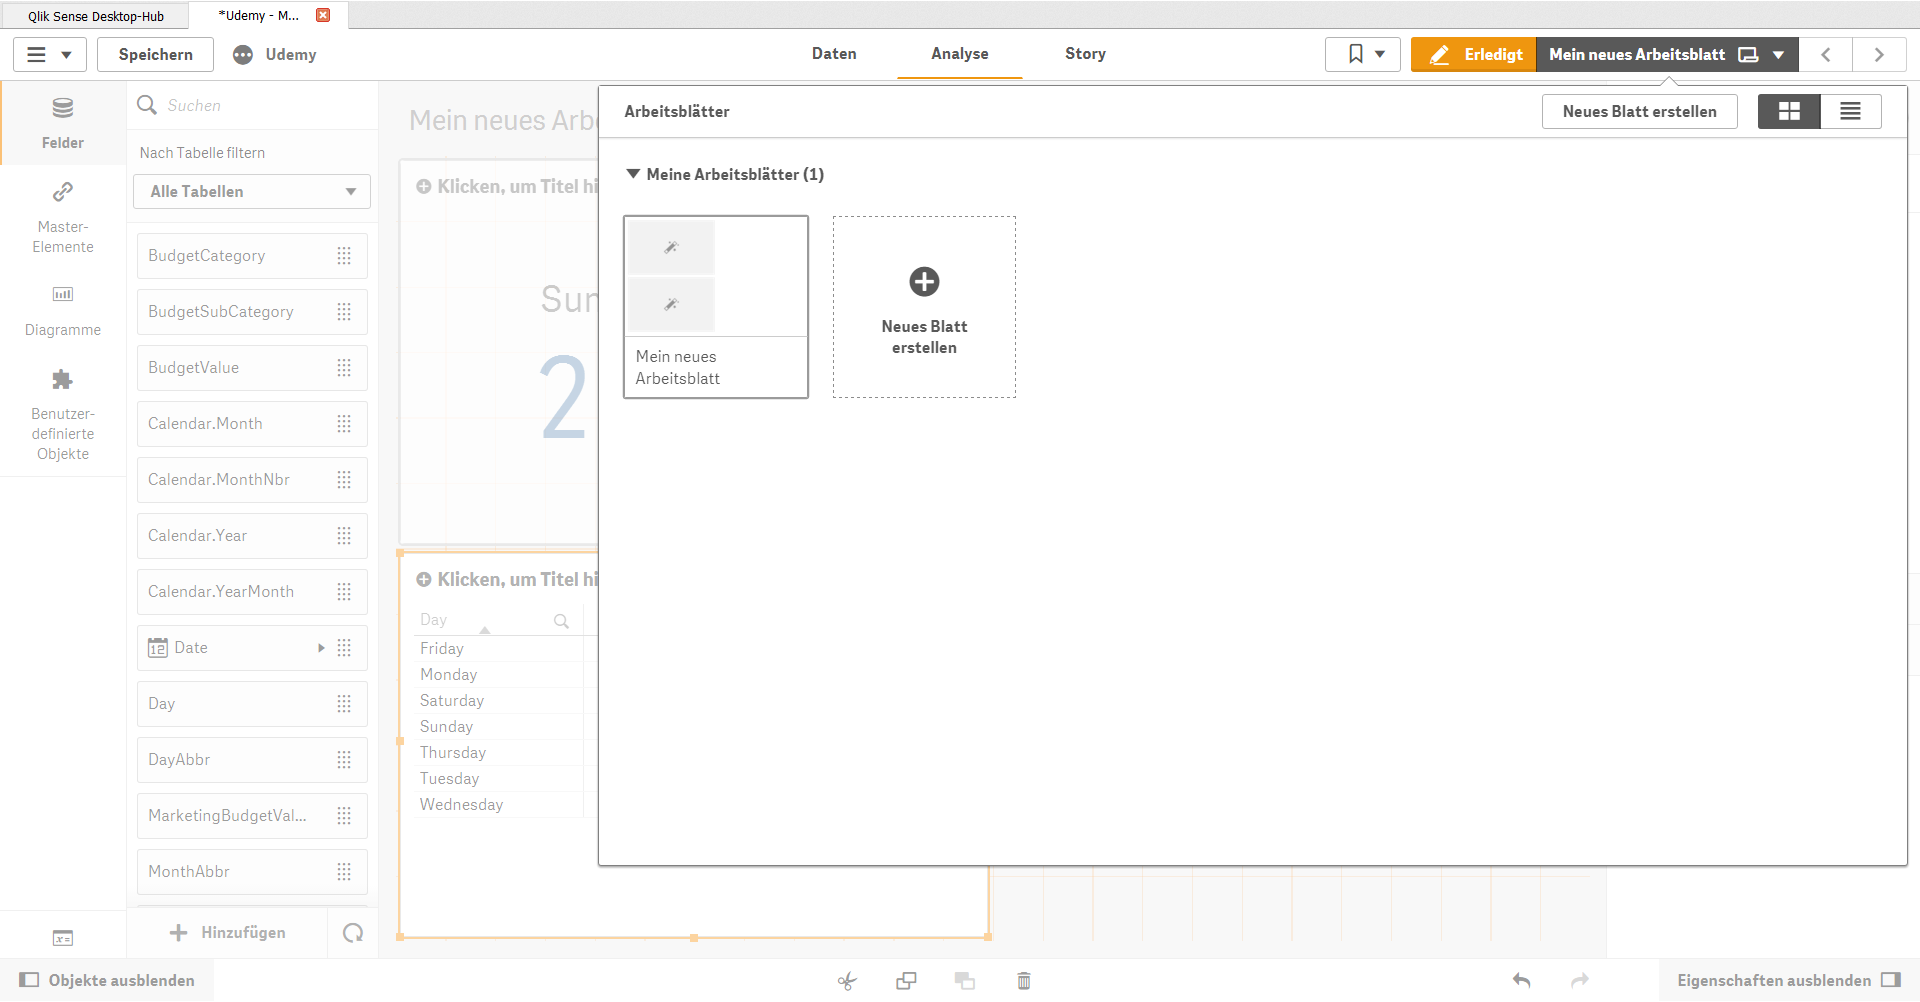
\includegraphics[scale = 0.3]{attachment/chapter_3/Scc017}
	\caption{}
	\label{fig:Scc017}
\end{figure}

Die \gls{g_QlikSense} speichert die Daten für eine App mit allen Informationen zu den Arbeitsblättern in \gls{.qvf} Dateien. In \gls{g_QlikSense} Desktop ist der vordefinierte Pfad:
\begin{figure}[H]
	\centering
	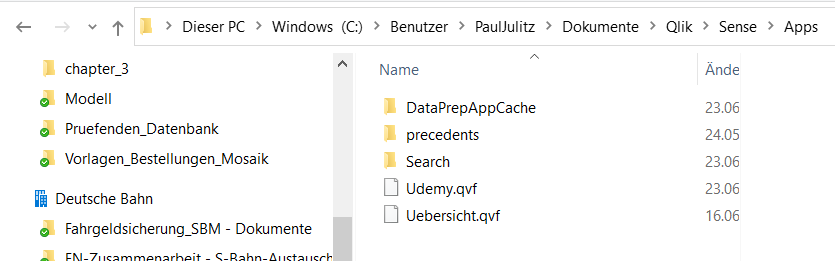
\includegraphics[scale = 0.3]{attachment/chapter_3/Scc018}
	\caption{}
	\label{fig:Scc018}
\end{figure}

\subsubsection{Selection}
Die QIX Engine agiert über Associationen. Tabellen werden über Schlüssel verbunden. Filter werden auf das gesamt Datenmodell angewandt. Es gibt verschiedenen Farben, die die Auswahl markieren.

Alle möglichen Auswahlen erscheinen weiß (Possible). Wir ein oder mehre Auswahlen getroffen, so erscheinen diese in grün (Selected). Alle anderen Möglichkeiten erscheinen in einem leichten grau (Altnative). Durch das Assoziativ Modell werden alle andern Filter angepasst. Auch hier erscheinen alle möglichen Auswahlen in weiß (Possible). Die Möglichkeiten die nicht ausgewählt werden können, erscheinen in einem dunklen grau (Excluded)
\begin{figure}[H]
	\centering
	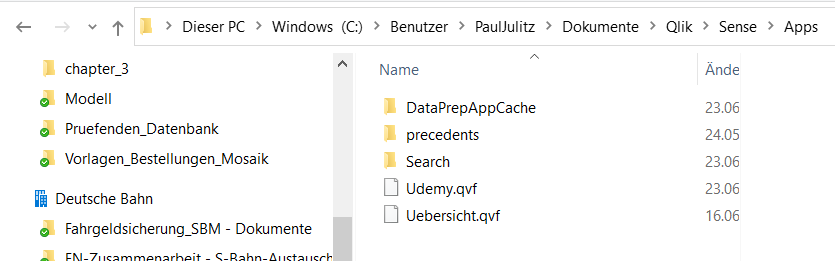
\includegraphics[scale = 0.3]{attachment/chapter_3/Scc018}
	\caption{}
	\label{fig:Scc018}
\end{figure}

\subsection{Qlik Key} 
\subsubsection{Composite Key} 
Die Assoziationen zwischen Tabellen kann auch manuell angestoßen werden. Die drei Begrifflichkeit sind Synonyme für den gleichen Sachverhalt.

Am folgenden Beispiel kann gezeigt werden, wie ein Composite Key verwendet wird, eine Kombination von Felder aus einer Tabelle mit einem anderen Feld aus einer anderen Tabelle verbunden werden kann.
1) Zu erst werden die beiden Tabellen geladen.
\begin{figure}[H]
	\centering
	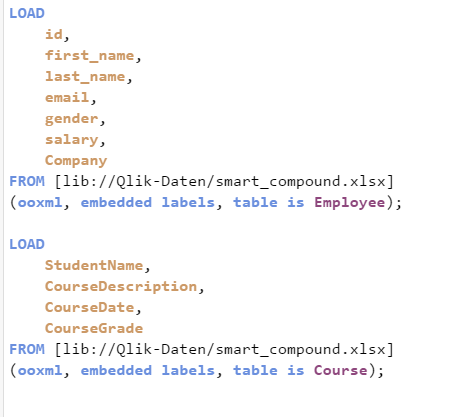
\includegraphics[scale = 0.3]{attachment/chapter_3/Scc019}
	\caption{}
	\label{fig:Scc019}
\end{figure}

2) Im Datenmanager kann keine Verbindung automatisch erzeugt werden, da keine Felder übereinstimmen.
\begin{figure}[H]
	\centering
	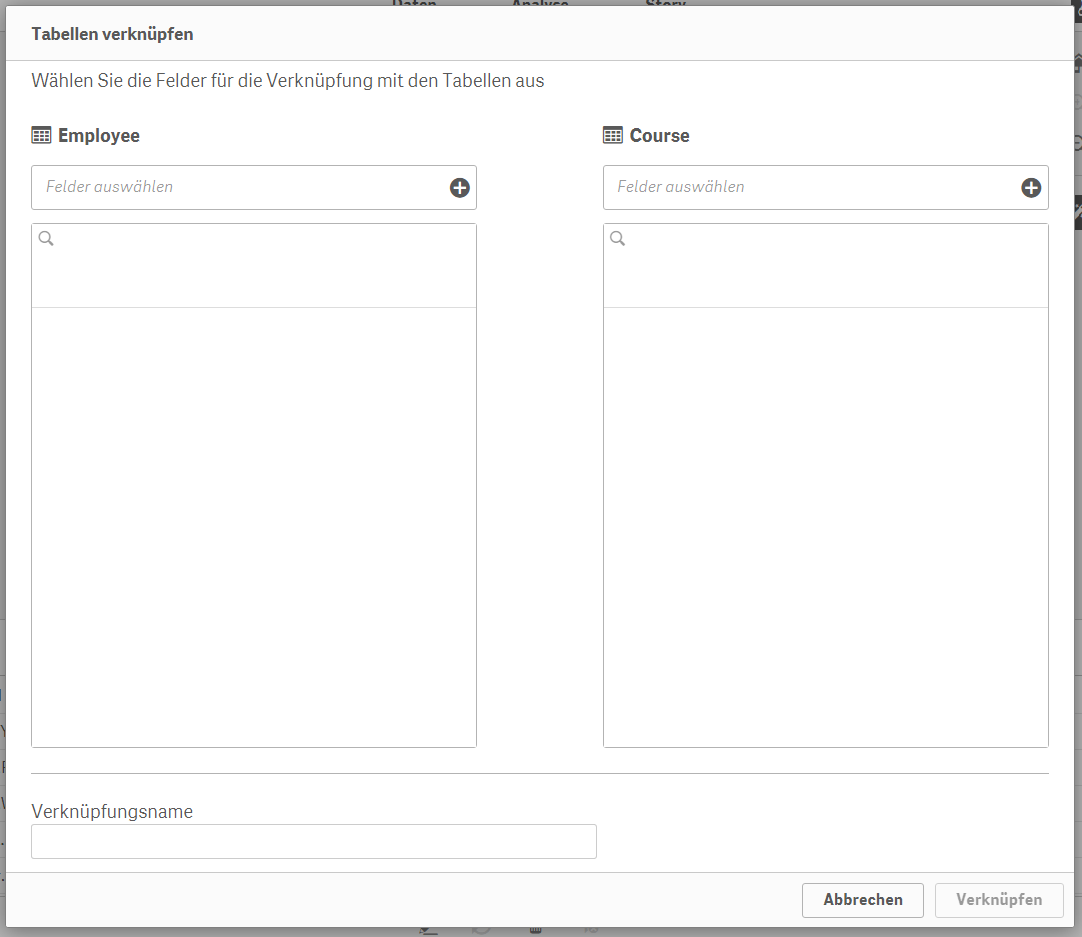
\includegraphics[scale = 0.3]{attachment/chapter_3/Scc020}
	\caption{}
	\label{fig:Scc020}
\end{figure}

3) Ein Composite Key kann jetzt direkt eingegeben werden. Dabei wird mit Hilfe eines Leerzeichen der [Vorname] und [Nachname] in der Employee Tabelle mit dem [StudentName] in der Course Tabelle verbunden.
\begin{figure}[H]
	\centering
	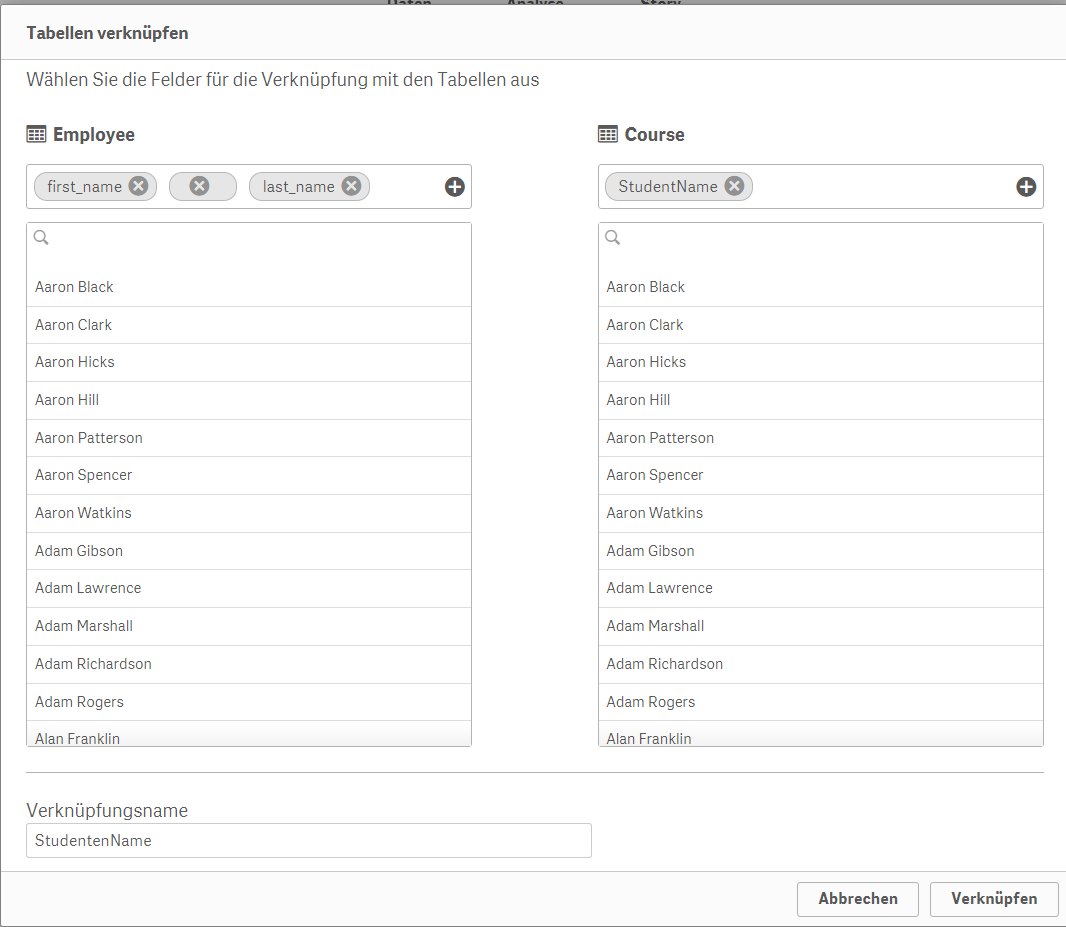
\includegraphics[scale = 0.3]{attachment/chapter_3/Scc021}
	\caption{}
	\label{fig:Scc021}
\end{figure}

4) Im Datenmanager wird die Verbindung jetzt rot angezeigt.
\begin{figure}[H]
	\centering
	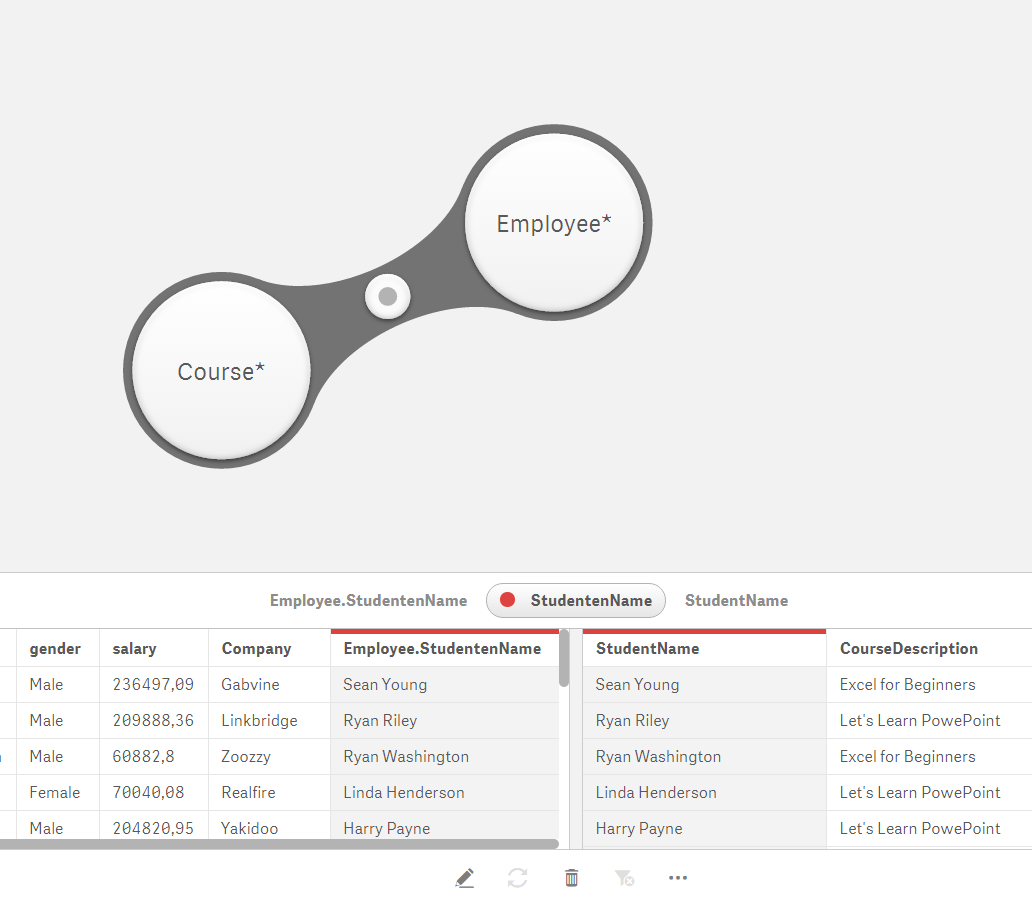
\includegraphics[scale = 0.3]{attachment/chapter_3/Scc022}
	\caption{}
	\label{fig:Scc022}
\end{figure}


5) Sheet Composite Key
\begin{figure}[H]
	\centering
	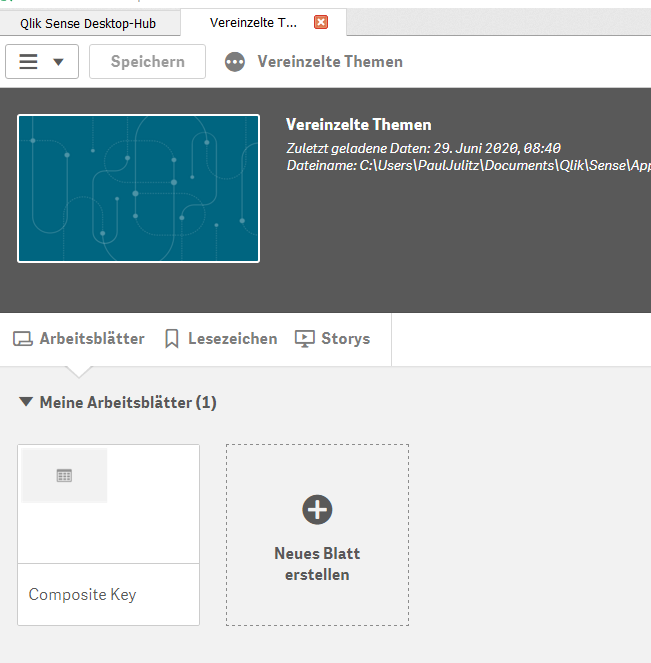
\includegraphics[scale = 0.3]{attachment/chapter_3/Scc023}
	\caption{}
	\label{fig:Scc023}
\end{figure}
Die App hat jetzt alle relevanten Daten geladen. Als nächstes kann ein Datenblatt angelegt werden. Dabei beinhaltet die App das Datenmodell und die Sheets geben Auskunft über die Visualisierungen.

6) Als Objekt der Wahl wird in dem Beispiel eine Tabelle eingefügt.
\begin{figure}[H]
	\centering
	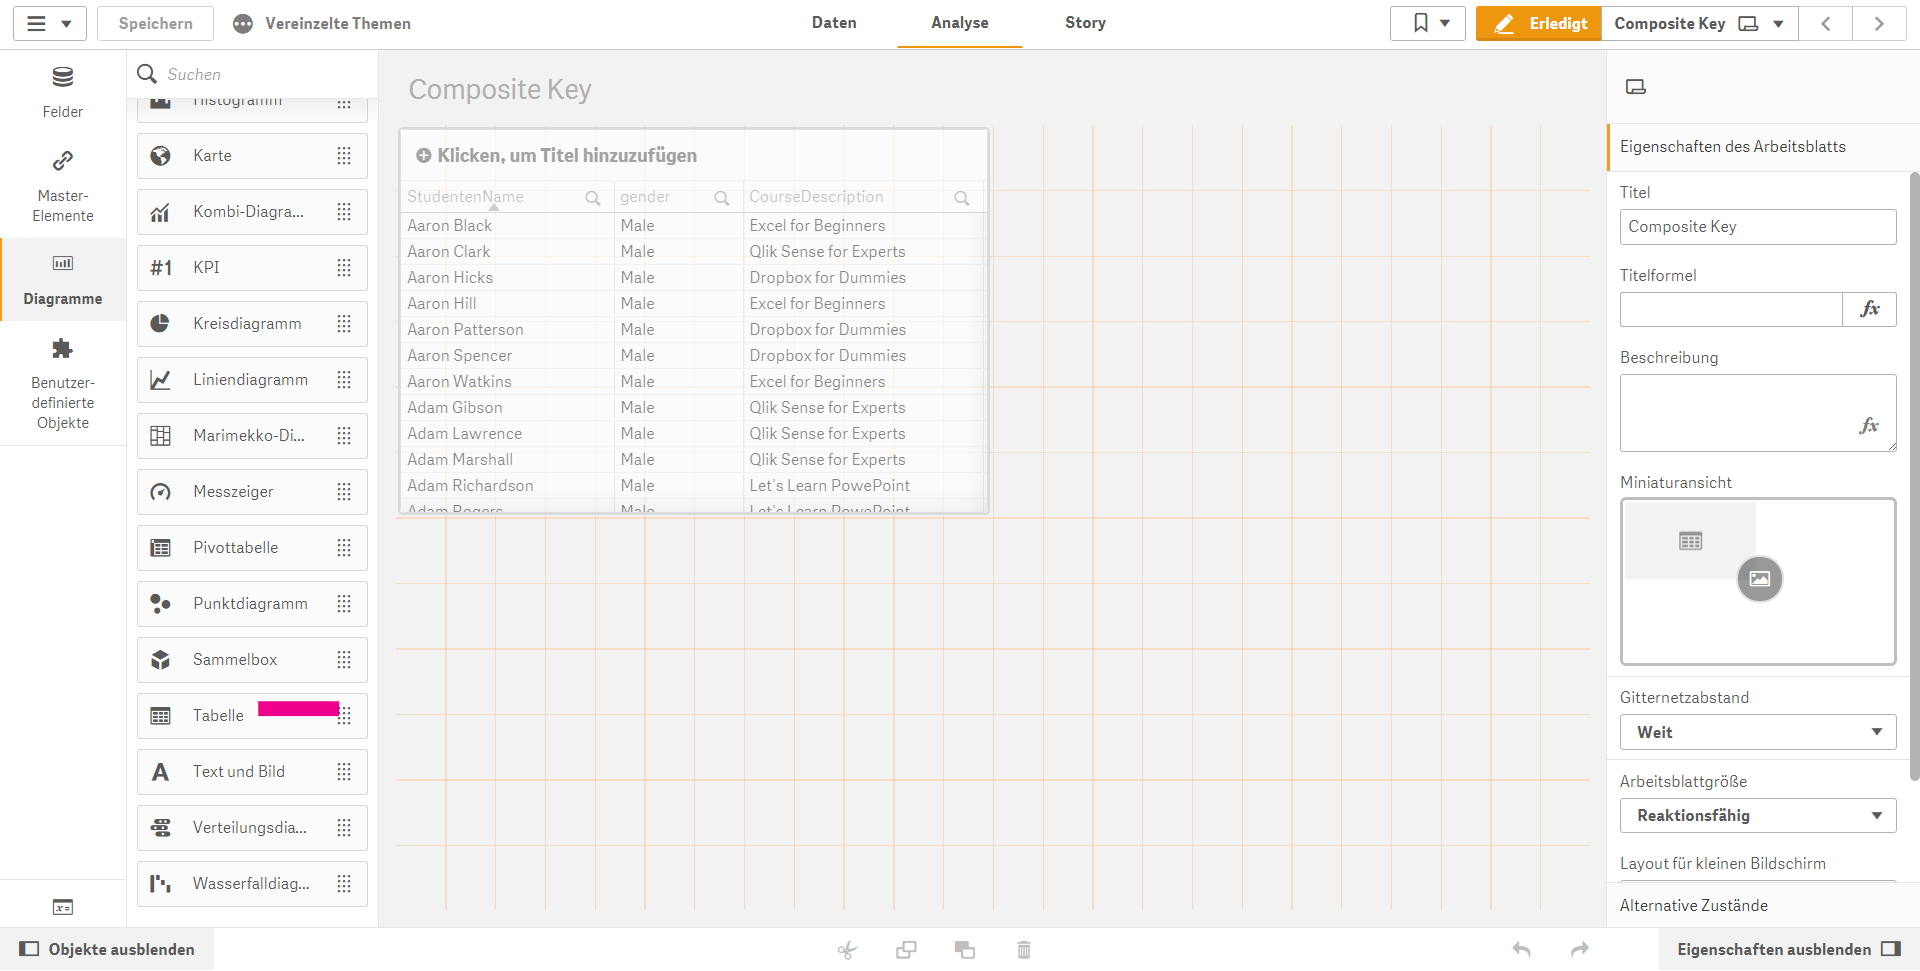
\includegraphics[scale = 0.3]{attachment/chapter_3/Scc024}
	\caption{}
	\label{fig:Scc024}
\end{figure}
7) Anhand der Verknüpfung [StudentenName] kann das Feld [CourseDescripton] von der Tabelle [Course] mit [Gender] von der Tabelle [Compony] in Verbindung gesetzt werden.
\begin{figure}[H]
	\centering
	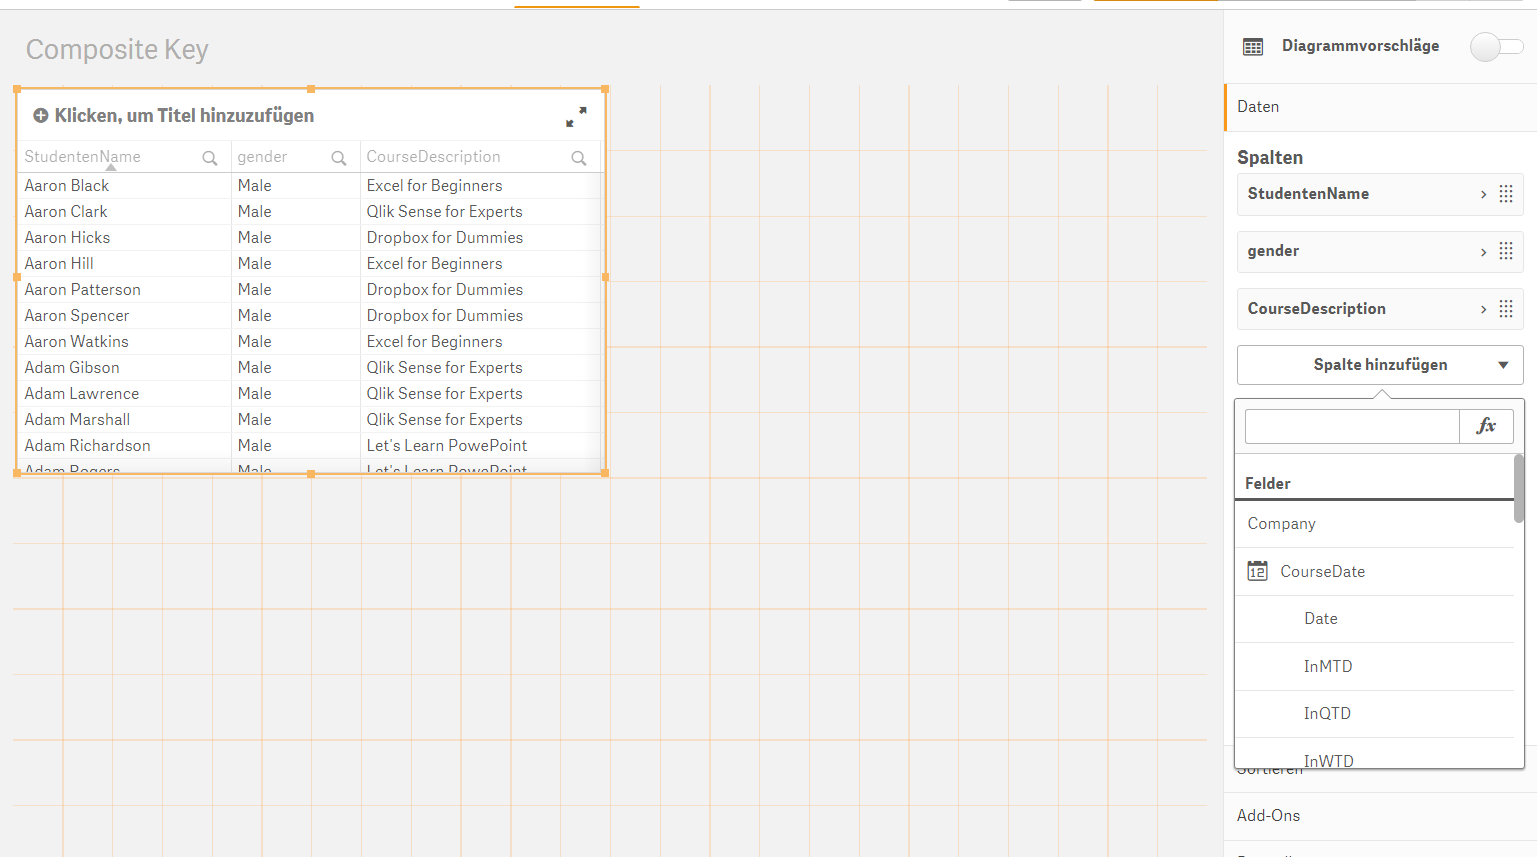
\includegraphics[scale = 0.3]{attachment/chapter_3/Scc025}
	\caption{}
	\label{fig:Scc025}
\end{figure}

Ein Composite Key kann auch direkt über den Daten Editor erstellt werden. Dabei wird die Spalte direkt über das \bl{Load} Statment abgeändert.

\begin{figure}[H]
	\centering
	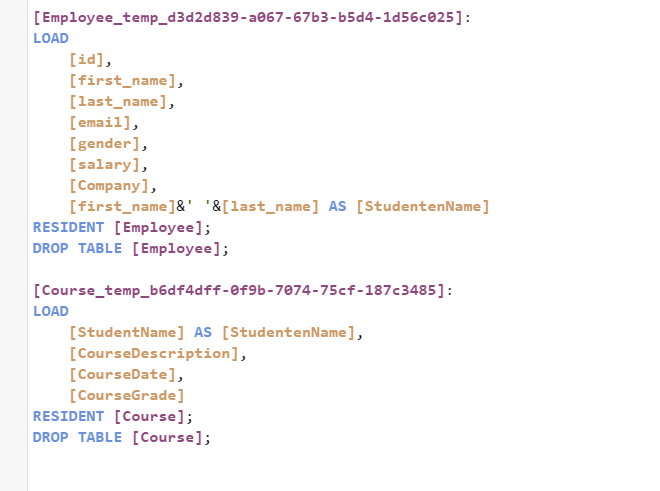
\includegraphics[scale = 0.3]{attachment/chapter_3/Scc028}
	\caption{}
	\label{fig:Scc028}
\end{figure}
Die Spalte [First Name] und [Last Name] wir verbunden und über \bl{as} als neue Spalte definiert.



\subsubsection{Synthetic Key}
Ein synthetischer Schlüssel wird erstellt, wenn zwei oder mehrere Felder in einer odere mehreren Tabellen gleich sind. 
\begin{figure}[H]
	\centering
	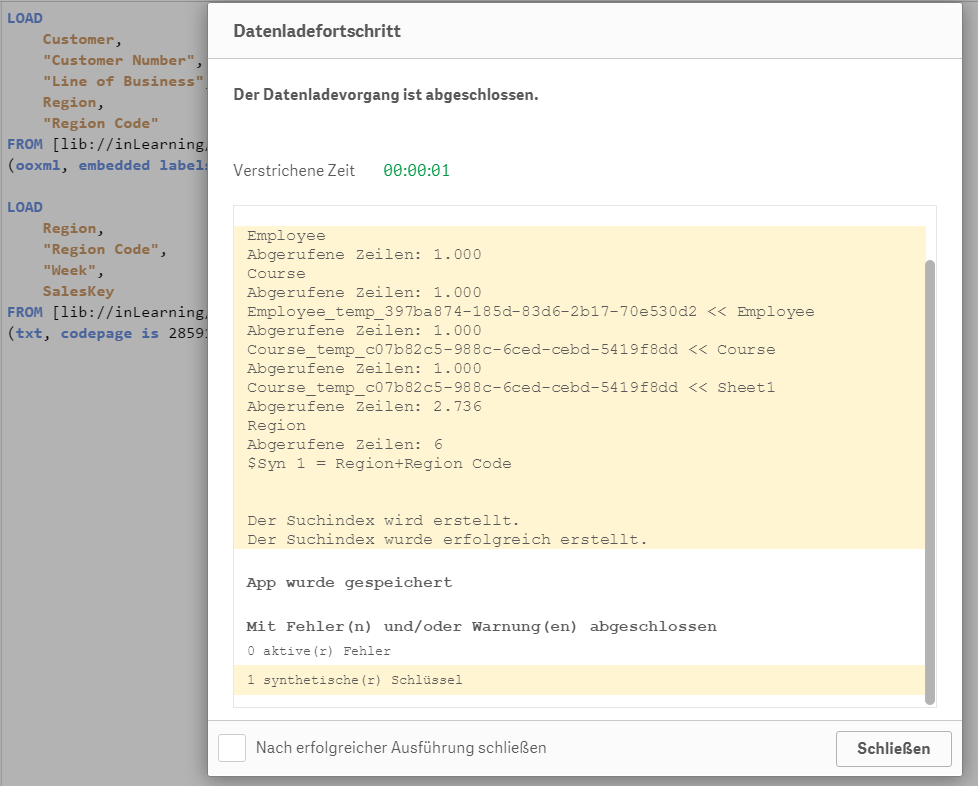
\includegraphics[scale = 0.3]{attachment/chapter_3/Scc026}
	\caption{}
	\label{fig:Scc026}
\end{figure}

Im gewählten Beispiel sind die Felder \textit{[Region]} und \textit{[Regio Code]} in zwei Tabellen gleich. \gls{g_QlikSense} erstellt eine Synthetic Tabelle \textit{$\$$Syn 1 Tabele}. Diese enthält das Feld \textit{$\$$ Syn1]}, und \textit{[Regio]} und \textit{[Regio Code]}. 
\begin{figure}[H]
	\centering
	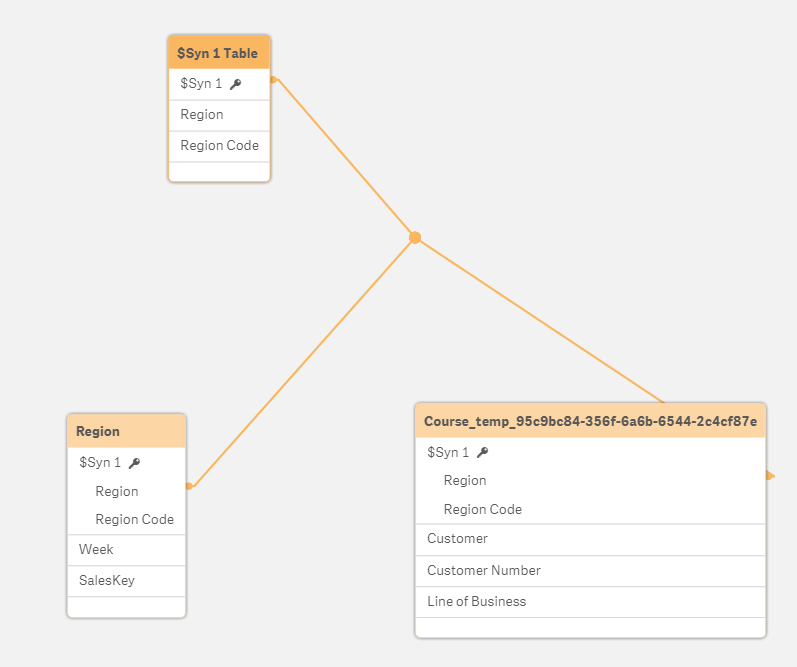
\includegraphics[scale = 0.3]{attachment/chapter_3/Scc027}
	\caption{}
	\label{fig:Scc027}
\end{figure}
Gleiches wird auch in den anderen Tabellen angelegt, obwohl diese nur über den synthetischen Schlüssel verbunden sind.\\
Sind Tabellen identisch, so werden diese verbunden und erscheinen im Modell als eine Tabelle. 
\subsubsection{Speicherung}
Damit Qlik effizient und schnell Berechnungen durchführen kann, werden alle geladenen Tabellen in zwei Typen gespeichert. Die eigentlichen Datentabellen und die Symboltabellen. Jeder Tabellenspalte wird eine Symboltabelle zugeordnet. In diesen gibt es zwei Spalten, die Pointer und Daten Spalte. Die Daten Spalte greift alle unterschiedlichen Werte einer Spalte auf. Die Anzahl der Zeilen bestimmt die Größe des Pointers. Dieser wird binär dargestellt. Qlik geht hier platzsparend vor. Der Pointer ist nämlich nur so lang - verbraucht nur so viele Stelle, wie benötig wird. Gibt es vier unterschiedliche Werte, so ist der Pointer drei Stellen lang - drei Bit
\begin{table}
	\centering 
	\begin{tabular}{cc}
		Pointer & Value \\ \hline
		000 & aa\\ 
		001 & asdf\\ 
	\end{tabular} 
\end{table}  

\section{Python Connection}
\begin{lstlisting}[style=python]
	\item Maschine Learning with Qlik: https://youtu.be/7E944kz1l5s
	\item https://developer.qlik.com/garden/5af5217ab2606a3c2c1f4d1d
	\item 
\end{lstlisting}
